Pour une expérience visuelle optimale, vous pouvez choisir d’utiliser un thème clair ou un thème foncé avec l’application.

\begin{multicols}{2}
\begin{figure}[H]
	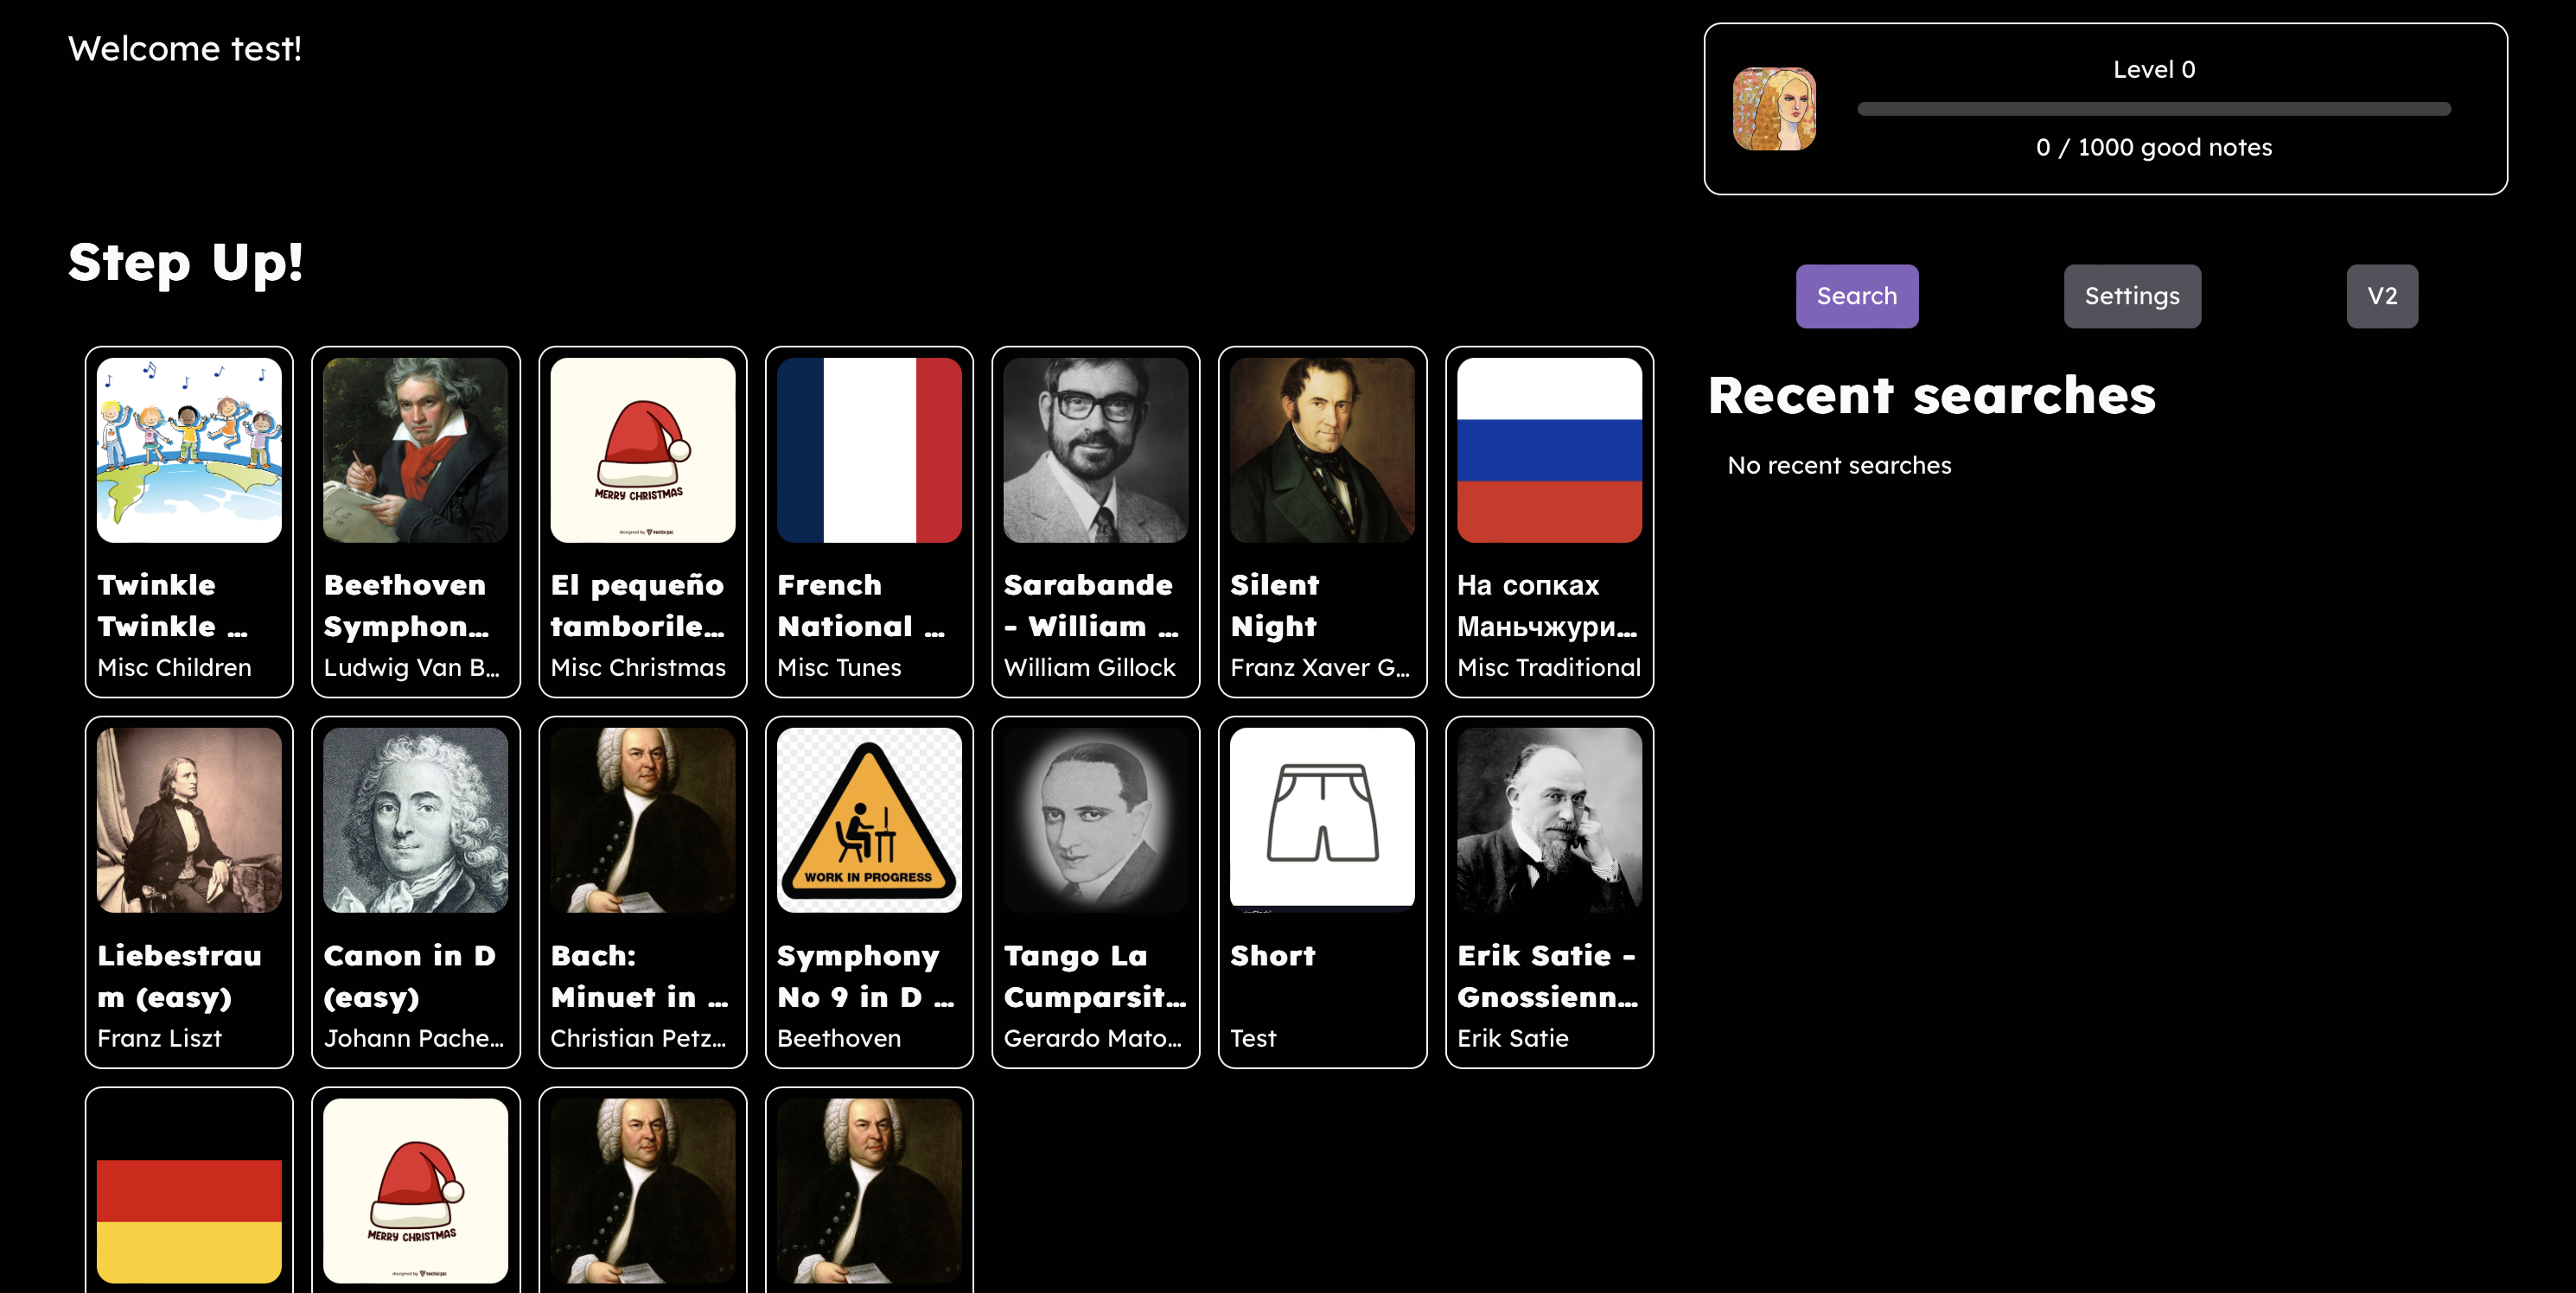
\includegraphics[width=\linewidth]{../\dir/guide/settings/dark.png}
	\caption{Theme foncé}
\end{figure}
\begin{figure}[H]
	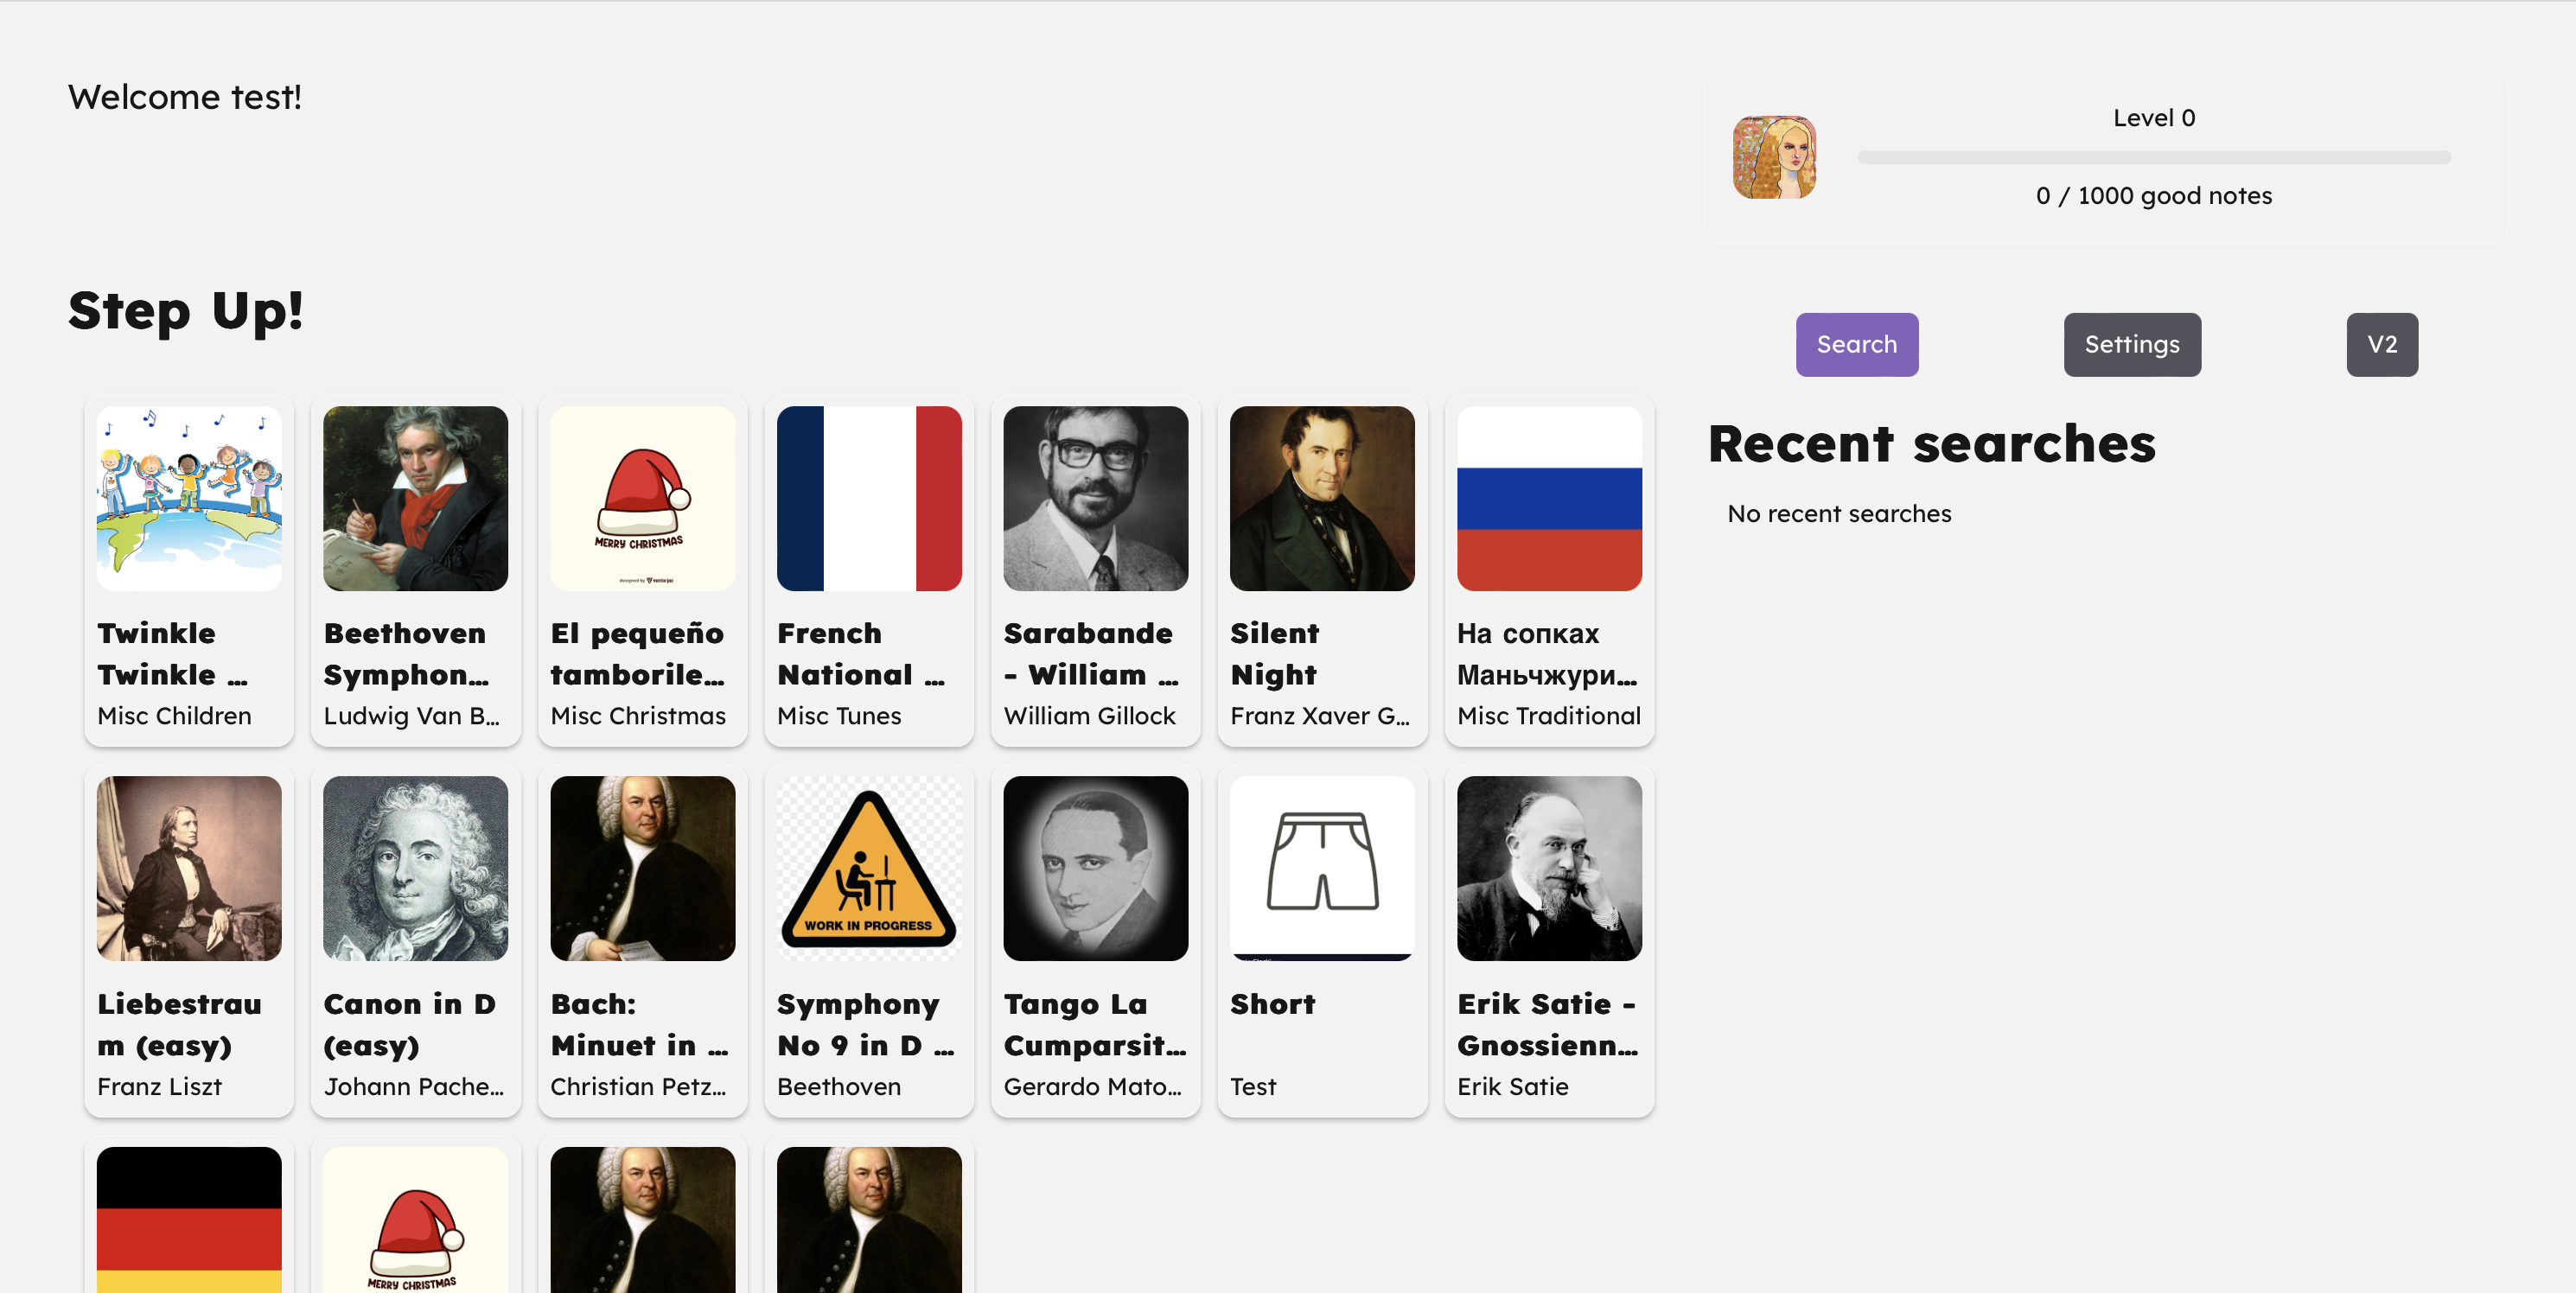
\includegraphics[width=\linewidth]{../\dir/guide/settings/light.png}
	\caption{Theme clair}
\end{figure}
\end{multicols}

Pour choisir quel thème utiliser, cliquez sur le bouton “Réglages” depuis votre page personnelle (Voir Capture \ref{fig:access-settings-theme}).

\begin{figure}[H]
	\begin{subfigure}[b]{0.7\textwidth}
		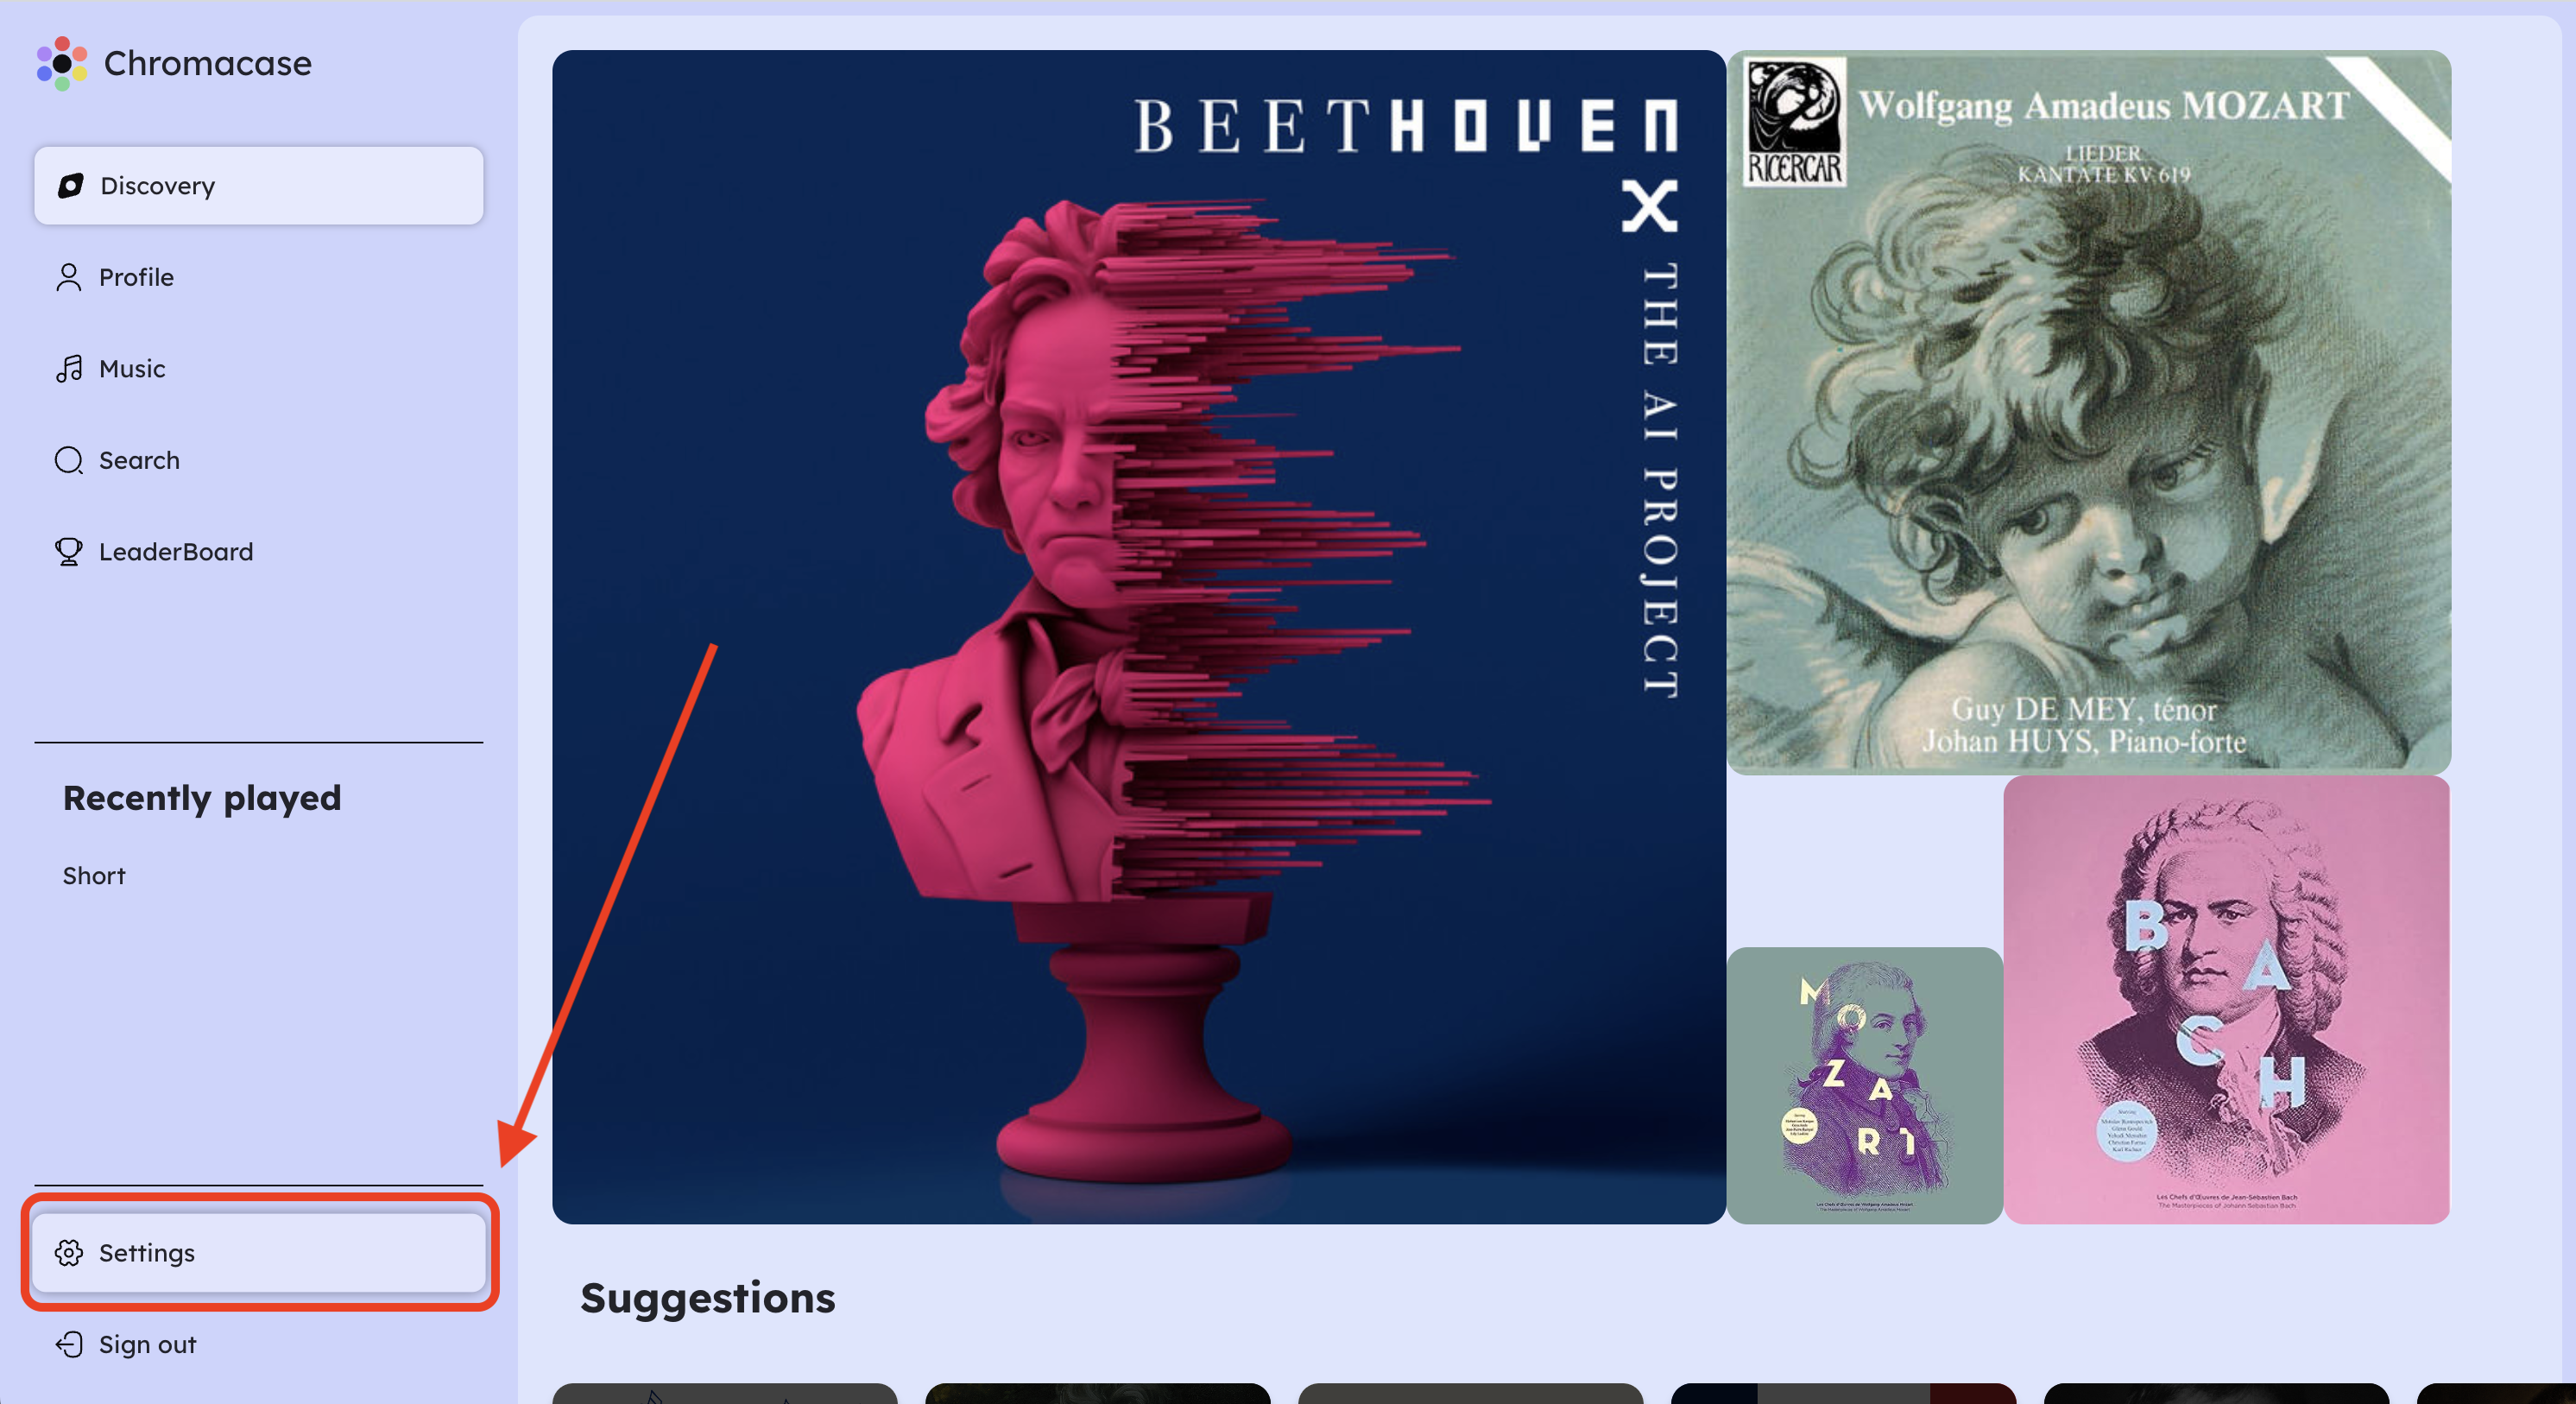
\includegraphics[width=\linewidth]{../\dir/guide/settings/access-settings.png}
		\caption{Version navigateur}
	\end{subfigure}
	\begin{subfigure}[b]{0.25\textwidth}
		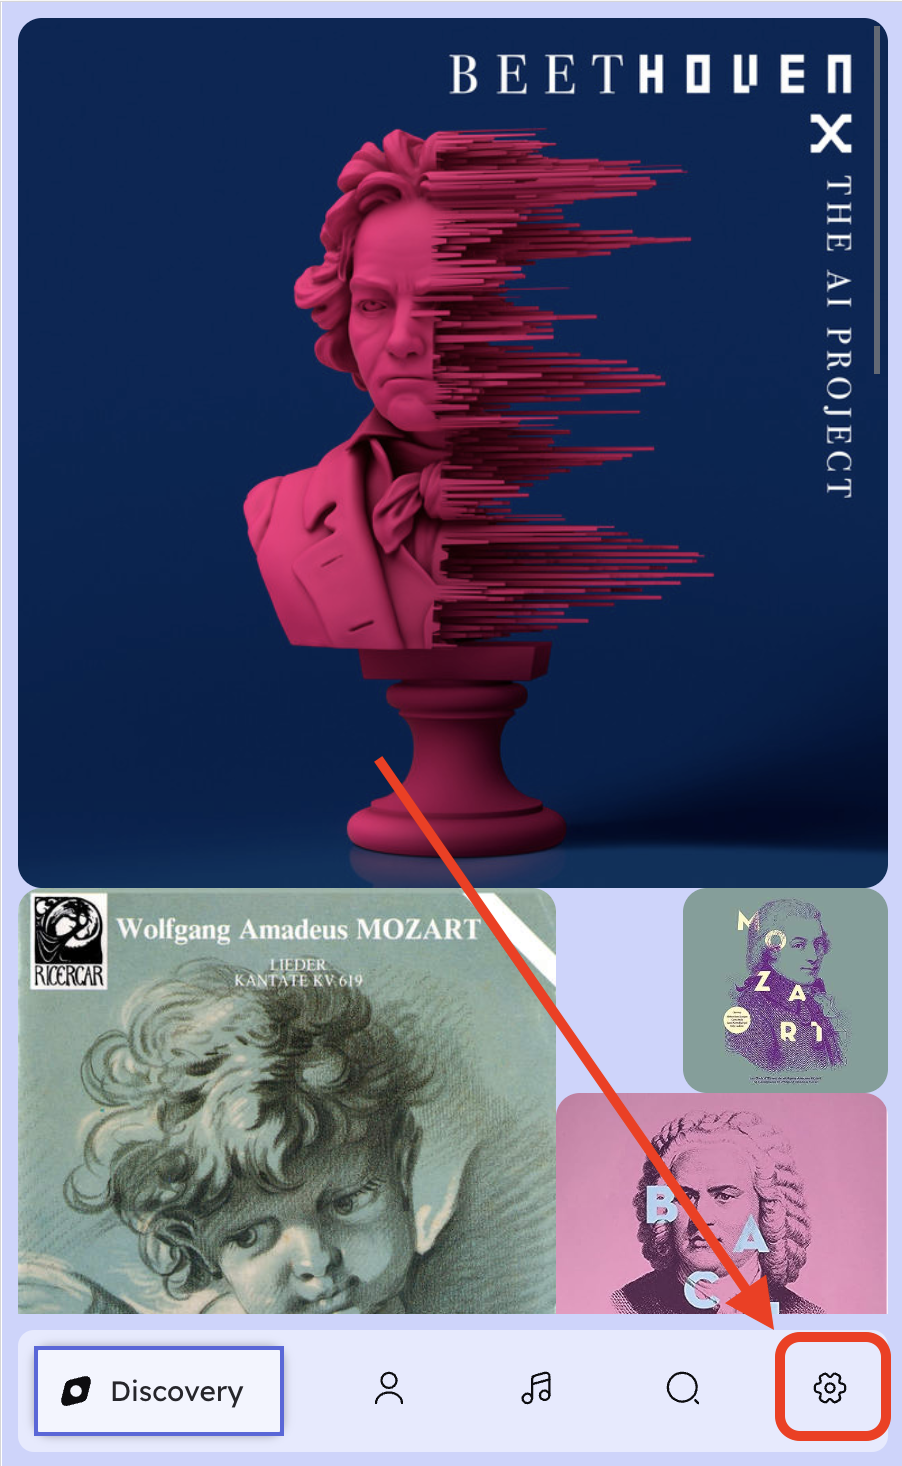
\includegraphics[width=\linewidth]{../\dir/guide/settings/access-settings-mobile.png}
		\caption{Version mobile}
	\end{subfigure}
	\caption{Accéder aux reglages}
	\label{fig:access-settings-theme}
\end{figure}
\begin{figure}[H]
	\begin{subfigure}[b]{0.7\textwidth}
		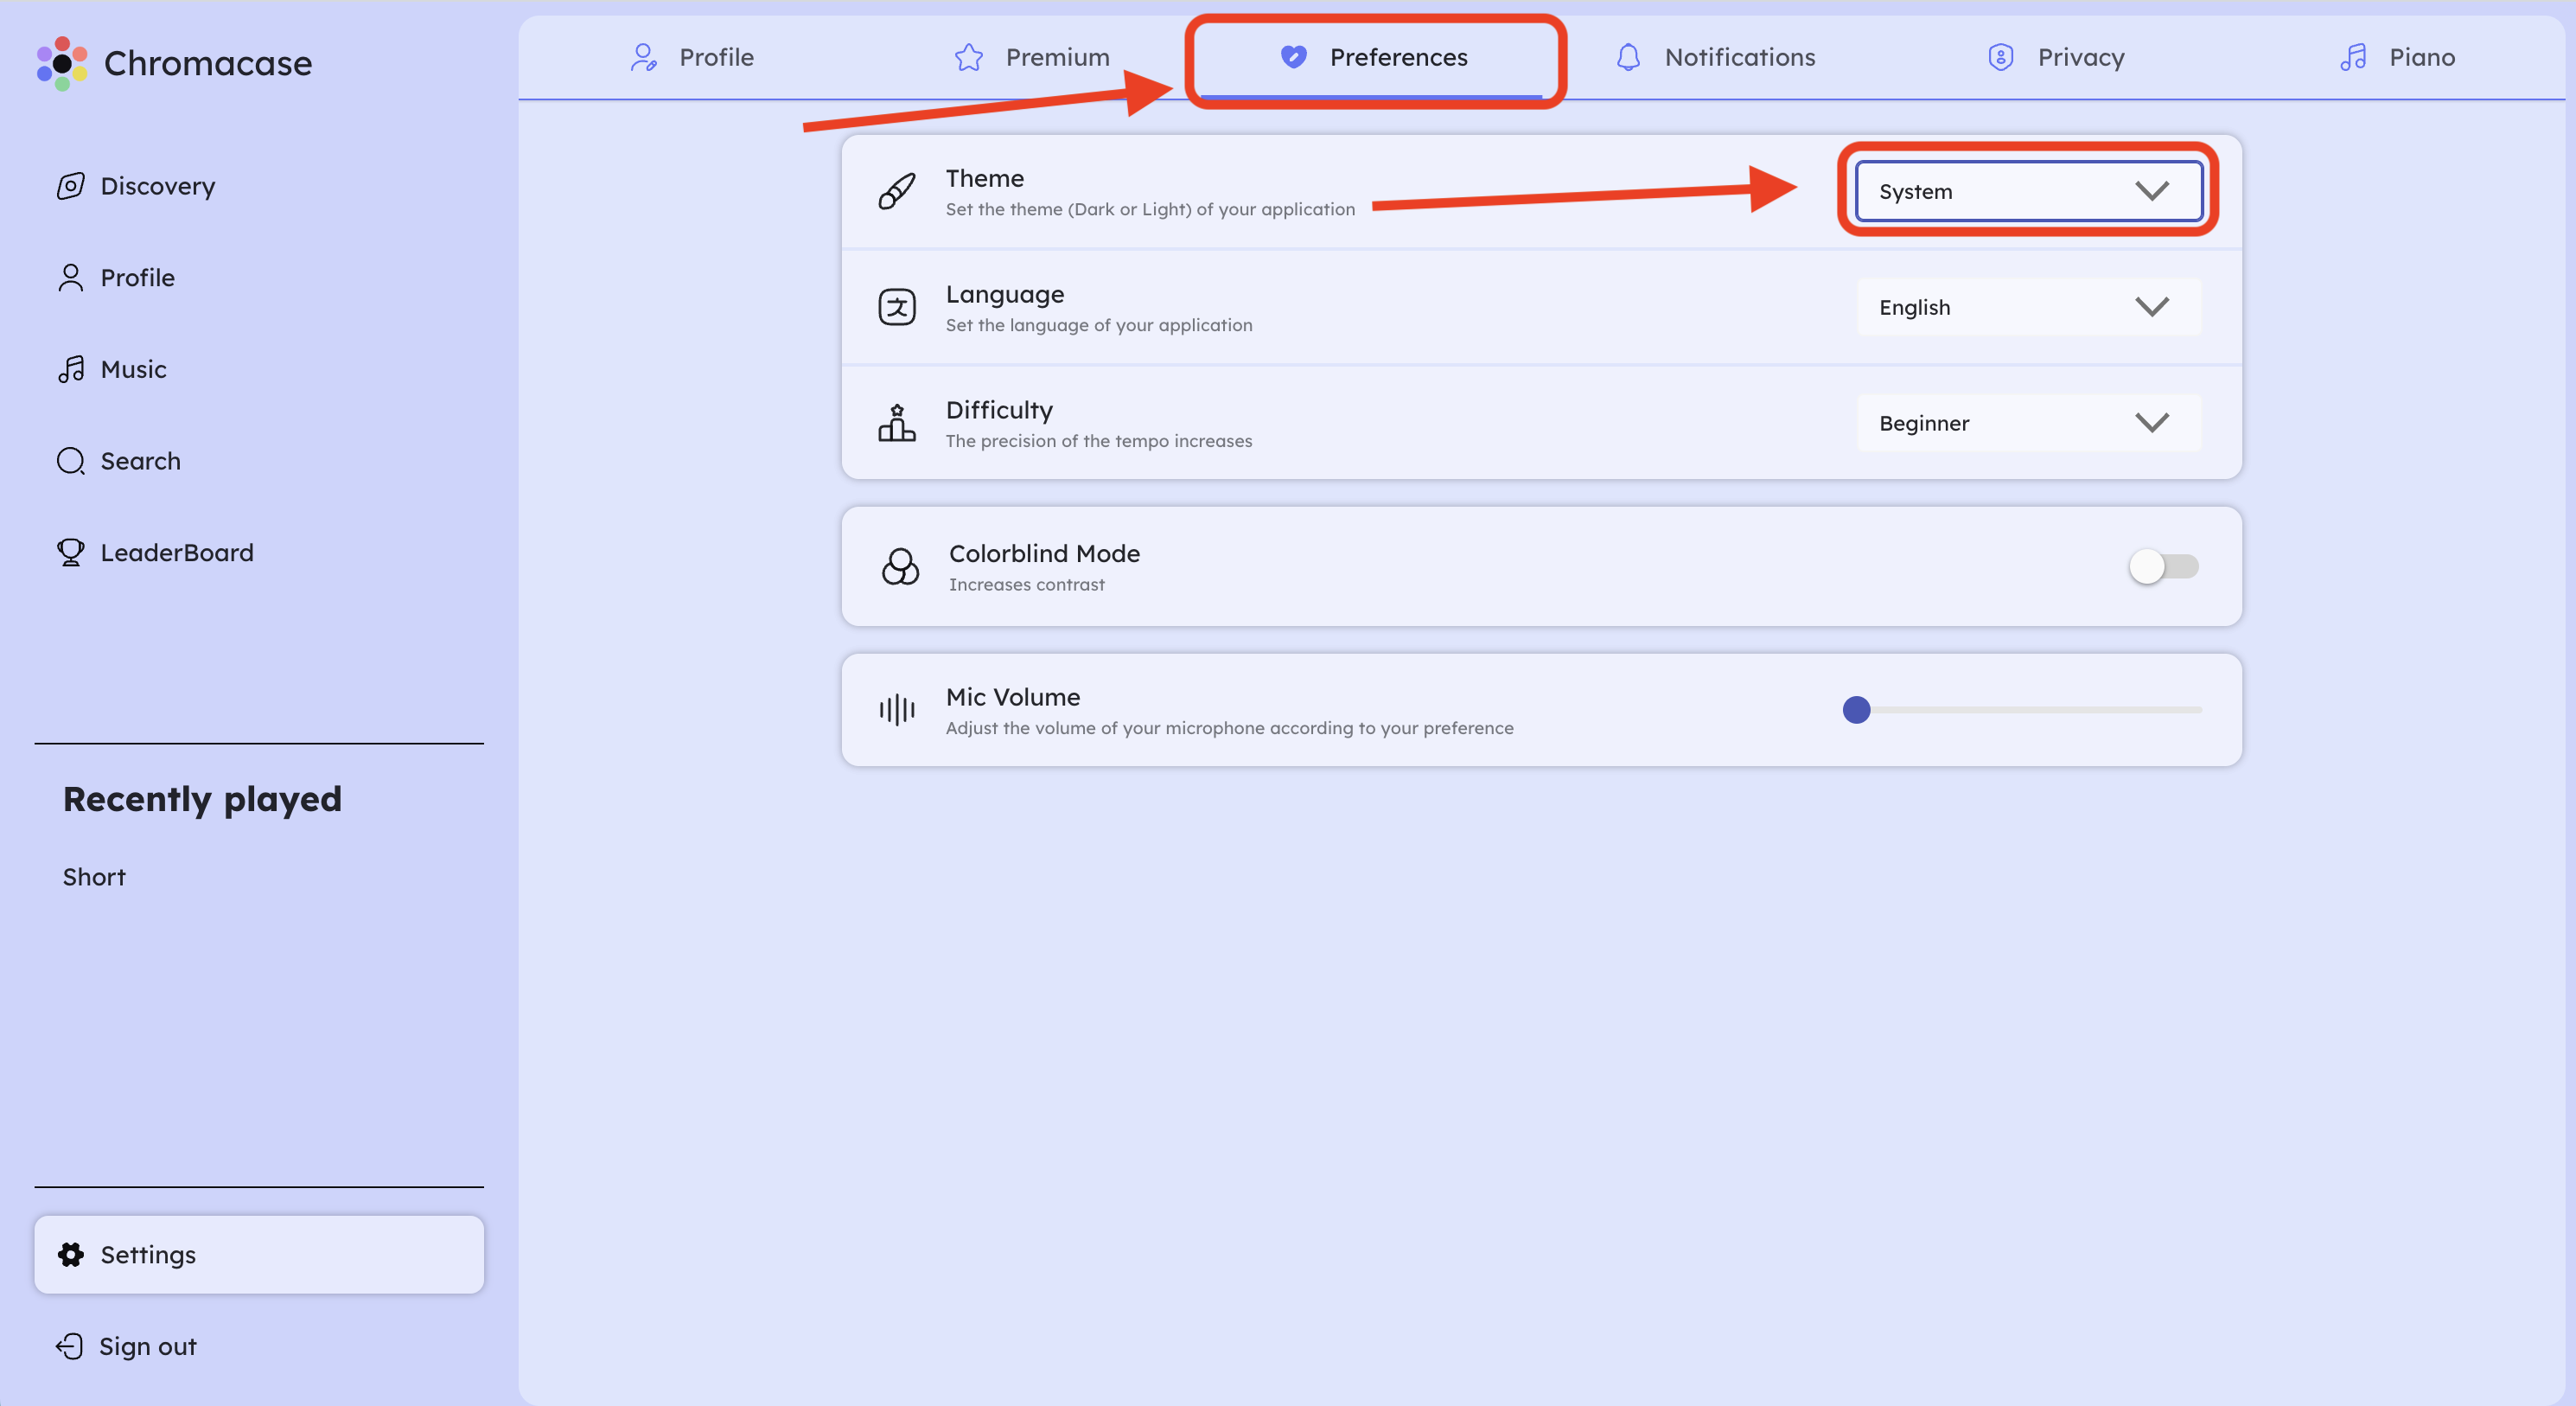
\includegraphics[width=\linewidth]{../\dir/guide/settings/change-theme.png}
		\caption{Version navigateur}
	\end{subfigure}
	\begin{subfigure}[b]{0.25\textwidth}
		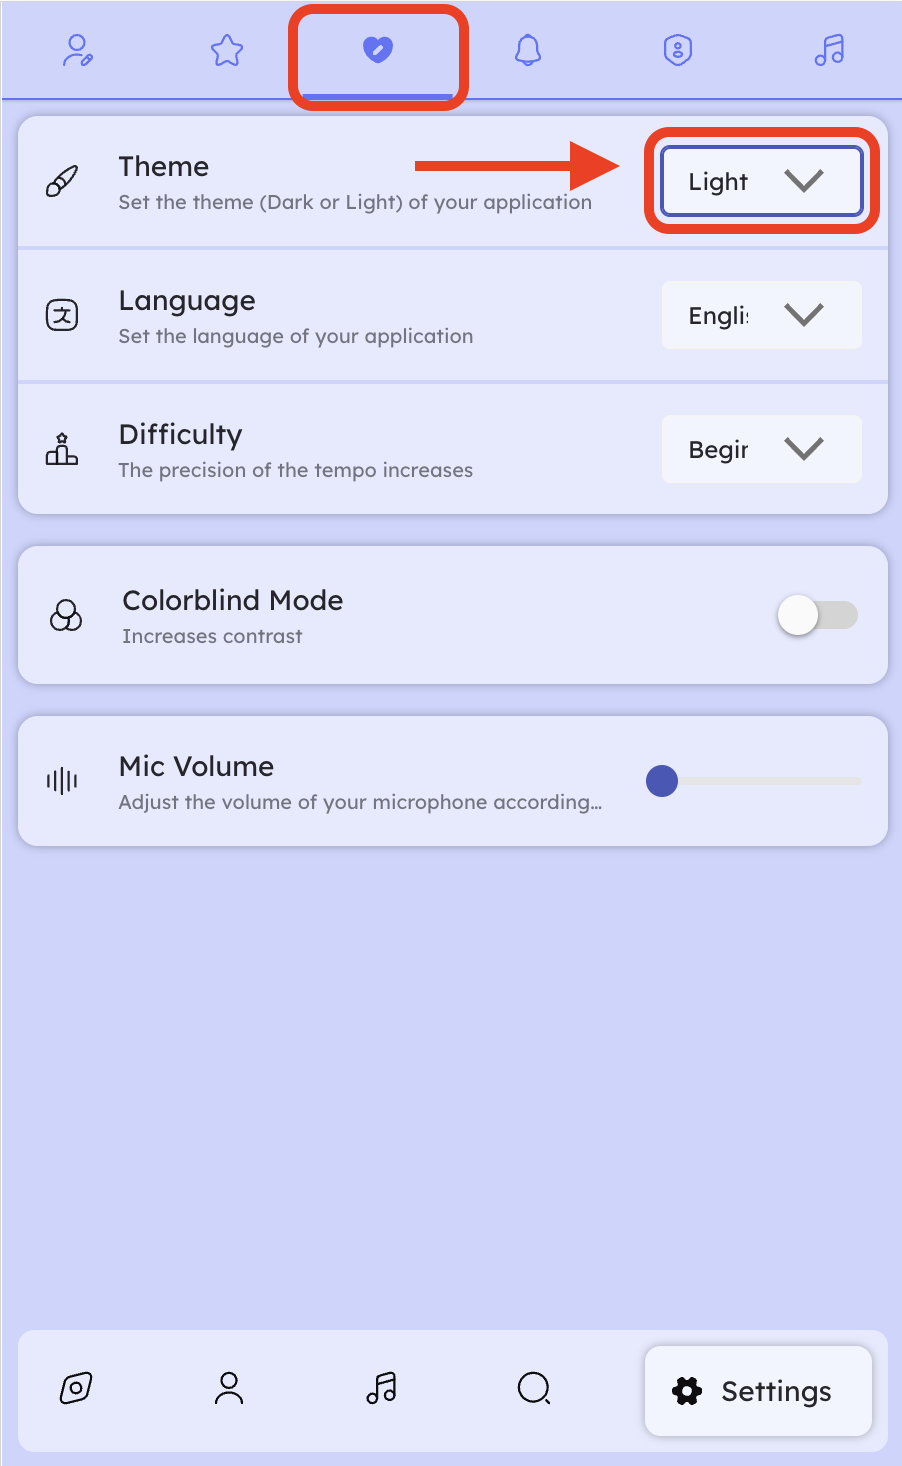
\includegraphics[width=\linewidth]{../\dir/guide/settings/change-theme-mobile.png}
		\caption{Version mobile}
	\end{subfigure}
	\caption{Selectionner le thème}
	\label{fig:change-theme}
\end{figure}

Sélectionnez l’onglet “Préférences”, et choisissez l’option de thème à utiliser (Voir Capture \ref{fig:change-theme}):

\begin{itemize}
 	\item Dark: Thème foncé
 	\item Light: Thème clair
 	\item Système: Utilise les réglages du navigateur
\end{itemize}
